\section*{Introduction}
The task was to implement an Finit State Machine in Simulink.
Afterwards this Finit State Machine is to be tested for its requirements.
Finally code should be generated and loaded onto the Arduino board. 

\section{Requirements}
In the next Subsections \ref{subsec:prio}, \ref{subsec:func} and \ref{subsec:missing} the requirements are explained in detail.


	\subsection{Order of Priorities} \label{subsec:prio}
	In this subsection the requirements are sorted according to their priorities.
		\begin{enumerate}
			\item \textbf{Unlocking}\\
				This is the core of the task and so the most important requirement.
			\item \textbf{Locking}\\
				It is necessary to return to the locked state.
			\item \textbf{Sampling}\\
				With a sampletime of 10ms you do not have to debounce the inputs. In this case is sampling important.							
			\item \textbf{Wrong Sequence}\\
				This requirement makes it difficult to crack the code using the brute force method.
			\item \textbf{Input Handling}\\
				This is a nice feature and can be useful if you have mistyped.
			\item \textbf{State}\\
				It would be a nice feature to see the current state. But it is not essential.		
			\item \textbf{Keypad}\\
				It is absolutely irrelevant whether the numbers are compared as integers between 0-9 or as ACII integers between 48 - 57.
%			\item Voltage Monitoring
		\end{enumerate}	
The Voltage Monitoring is an own requirement. Because it has no connection with the remaining requirements.
	
	
	\subsection{Funcional and non functional requirements}\label{subsec:func}
	The requirements from the Word-document where splited in functional and non functional requirements.
		\subsubsection{Functional}
			\begin{description}
				\item [Unlocking] Configurable sequence and the change of the output is functional\\
				\item [Wrong Sequence] To blocking the entry for 5s after three wrong sequence entry is functional
				\item [State] Make the current state visible is a functional demand
				\item [Input Handling] To detect input changes is functional															
				\item [Voltage Monitoring] Is a standart system function
			\end{description}
		\subsubsection{Non functional}
			\begin{description}
				\item [Unlocking] It is non functional to enter the sequence by the button \# \\
				Should the output be true or false after the correct sequence is non functional
				\item [State] To make the state by an output visible is non functional
				\item [Sampling] It is a resource requirement
				\item [Locking] It is not functional with which button the lock can be closed
				\item [Keypad] It is an additional requirements, an other possibility whould be a wheel or a fingerprint scanner\\
				It is also not a system requirement whether the data comes in ascii or binary or whatever
				\item [Voltage Monitoring] The power source is not a system requirement\\
				A system requirement whould be a portable power source		
			\end{description}

	\subsection{Missing requirements}\label{subsec:missing}
	Some missing requirements are listed here:
	\begin{itemize}
		\item Minimum an maximum voltage
		\item To change the sequence while running the system
		\item The power source have to be portable or not
		\item Alarmsystem in case of wandals
		\item Size of sequence
		\item Area of use
	\end{itemize}

	\section{Stateflow implementation}
	Based on the previously defined requirements the state machine of the numeric sequence lock shall be implemented in Simulink using stateflow. This task begins with defining the needed cases and then working on the transitions between said cases.
		\begin{figure}[H]
				\centering
				\includegraphics[width=0.7\textwidth]{figures/stateflow.png}
				\caption{stateflow implementation of the state machine}
				\label{fig:state}
		\end{figure} 

		\subsection{Statemachine detailed}
		In order to further understand the working of the models, each case will be briefly explained and reviewed. An overview is in Figure \ref{fig:state}.
		\\~\\
		\underline{INIT} \newline
		As the name implies, this state sets the initial condition for the lock. The fail counter is reset to zero and other initial settings such as the sequence length and the sequence key are set in here. The Transition to the next state is made immediately after setting all parameters, without any conditions.
		\\~\\
		\underline{LOCKED} \newline
		The system gets locked and the buffer for the user input is reset. The index i is used to keep track of how many digits were already entered. Again, the transition to the next state is done immediately after finishing all tasks without any conditions.
		\\~\\
		\underline{IDLE} \newline
		This state is used to wait for user inputs, other than that it serves no purpose. After a user input was detected, the transition to the READING state is made.
		\\~\\
		\underline{READING} \newline
		Here the detected input is stored in the previously declared buffer and the index is increased. If the index exceeds the sequence length, the state machine transitions to the CHECK state, if not, and the user input changes again (button was released) it moves back to the IDLE state and waits for the next digit.
		\\~\\
		\underline{CHECK} \newline
		In this state the machine waits for the user to activate the enter key to confirm the input. After receiving it the sequence is compared to the key and if it matches the machine moves to the UNLOCK state. If the sequence is wrong, it moves on to the WRONG\_CODE state.
		\\~\\
		\underline{UNLOCK} \newline
		This is the state in which, if there was an actual locking hardware attached, the system unlocks itself. After completing the unlocking phase, it moves back to the INIT state to reset the system.
		\\~\\
		\underline{WRONG\_CODE} \newline
		Here the fail counter is increased and if it exceeds the allowed fail attempts, it moves to the LOCKDOWN state. If the limit Is not yet reached the machine jumps back into the LOCKED state in order to allow another try. 
		\\~\\
		\underline{LOCKDOWN} \newline
		The system waits for 15 seconds before returning into the LOCKED state. In addition, the fail counter is reset.
		
		\subsection{Input translation}
		Since the Arduino later will receive ascii values for the available some sort if translation to the system must be implemented in order to feed the statemachine the correct inputs. This was done by creating a simple subsystem in Simulink, evident in Figure \ref{fig:check}.\\
		The different inputs are filtered by their ascii value and fed into their outputs. The star an the hashtag are rather obvious. The interval filters for the ascii value of all 10 digits and the resets them to values from zero to nine. 
			\begin{figure}[H]
					\centering
					\includegraphics[width=0.7\textwidth]{figures/check_input.png}
					\caption{check input subsystem in Simulink}
					\label{fig:check}
			\end{figure}
		
		
		\subsection{Testing}
		In order to test the system without its hardware a constant was attached to the input of the check input subsystem. This system is shown in Figure \ref{fig:test}. The constant got linked to multiple push buttons which made testing the functionality possible. 
			\begin{figure}[H]
					\centering
					\includegraphics[width=0.7\textwidth]{figures/testing_sim.png}
					\caption{Test structure of the sequence lock}
					\label{fig:test}
			\end{figure}
		All possible cases where tested and the system held up to the expectations. If the correct sequence was entered and the hashtag was pressed the system unlocked itself. The input of the ‘/’ character was ignored. After then pressing the start button the system was locked again. If the wrong sequence was entered the system returned into the IDLE state. If the wrong code was entered too many times the LOCKDOWN state was entered. However, the time the system spent in this state was way too short due to Simulink not simulating in real time.
		
		\subsection{Arduino implementation}
		After having a working model of the sequence lock the next step was to transfer the software onto the actual hardware, this time being an Arduino UNO with a numerical pad attached. Simulink shall automatically generate the required C code. For this purpose the number pad was attached to the Arduino as in Figure \ref{fig:ard_wir}.
			\begin{figure}[H]
					\centering
					\includegraphics[width=0.7\textwidth]{figures/arduino_wiring.png}
					\caption{pin assignment (Source: ECE MBD: Laboratory session)}
					\label{fig:ard_wir}
			\end{figure}
		The given template for the keypad was included into the Simulink model and the settings were adjusted in order to motivate Simulink to deploy the code onto the Arduino. Visible in Figure \ref{fig:ard_imp} and \ref{fig:settings}.
			\begin{figure}[H]
					\centering
					\includegraphics[width=0.7\textwidth]{figures/arduino_implementation.png}
					\caption{Implementation in simulink for arduino}
					\label{fig:ard_imp}
			\end{figure}
			\begin{figure}[H]
					\centering
					\includegraphics[width=0.7\textwidth]{figures/simulink_settings.png}
					\caption{simulink settings}
					\label{fig:settings}
			\end{figure}
		In addition, the compile mode has to be set to external. After that the model was deployed on the Arduino and was ready for testing. In order to check the correct working behavior, the same procedure as before was used. Only this time the buttons on the keypad where pressed as opposed to the ones in the Simulink model.

	
	
	\section{Voltage Monitoring}
	Due to the simplicity of the voltage monitoring requirements, no stateflow was implemented to do this. For this example were seted 3.3V as minimum  and as maximum 3.7V. In Figure \ref{fig:v_mon} is the implementation evident. The voltage input is compared with the minimum and maximum value. If the input value ist higher or lower then then a rectangular signal is emitted on the respective output. This signal is boolean and triggers all 0.5sec. \\
	Slight voltage fluctuations were neglected. Therefore no schmitt-trigger was realized. Therefore it could be that the output sometimes flashes only very quickly or a short time. 
		\begin{figure}[H]
			\centering
			\includegraphics[width=0.7\textwidth]{figures/v_monitor.png}
			\caption[Implementation of the voltage monitoring]{Implementation of the voltage monitoring\\ Source: Own presentation}
			\label{fig:v_mon}
		\end{figure}
	In Figure \ref*{fig:v_test} is a test setup for the voltage monitor. As input a sinus generator was used. The amplitude was 1.5V with an offset was 3.5V, so the middle between minimum and maximum. The frequence is $1^{rad}/_{sec}.$ The results of this test is visible in Figure \ref{fig:v_graph}.
		\begin{figure}[H]
			\centering
			\includegraphics[width=0.7\textwidth]{figures/v_monitor_testcase.png}
			\caption[Test structure]{Test structure\\ Source: Own presentation}
			\label{fig:v_test}
		\end{figure}
		
		\begin{figure}[H]
			\centering
			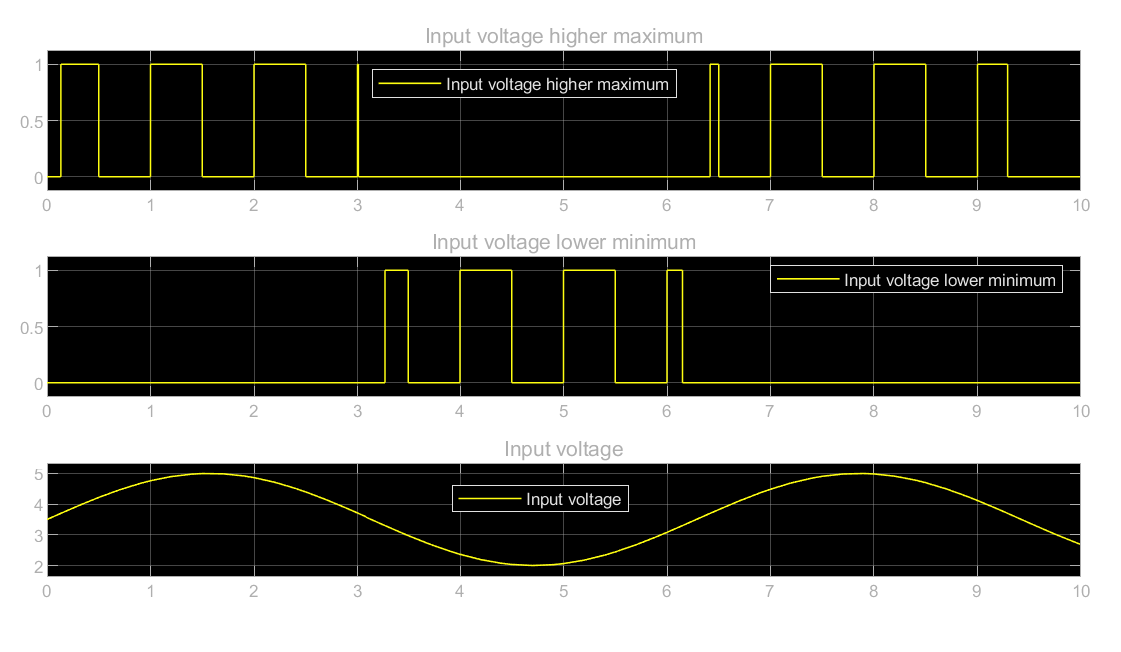
\includegraphics[width=0.7\textwidth]{figures/v_monitor_graph.eps}
			\caption[Plot of the in- and outputs]{Plot of the in- and outputs. The two upper plots are boolean depence of time. The third is voltagein dependence of time\\ Source: Own presentation}
			\label{fig:v_graph}
		\end{figure}
	
	
	
\section{Conclusion}
\todo{Ideas}
